\chapter{General-Purpose User Embeddings based on Mobile App Usage}

Tencent \\

\textbf{Reference:}~\cite{zhang2020general} 

\textbf{Keywords:} user behavior, embeddings, deep learning

\section*{Какую задачу решают авторы?}

Данныи об использовании пользователем мобильных приложений несут в себе много информации о его интересах (см. Рисунок~\ref{fig:behaviors}). 

Список установленных приложений, установки, удаления --- все это хорошие индикаторы как долгосрочных так и кратковременных интерсов пользователя. \\

\begin{figure}[ht]
  \centering
  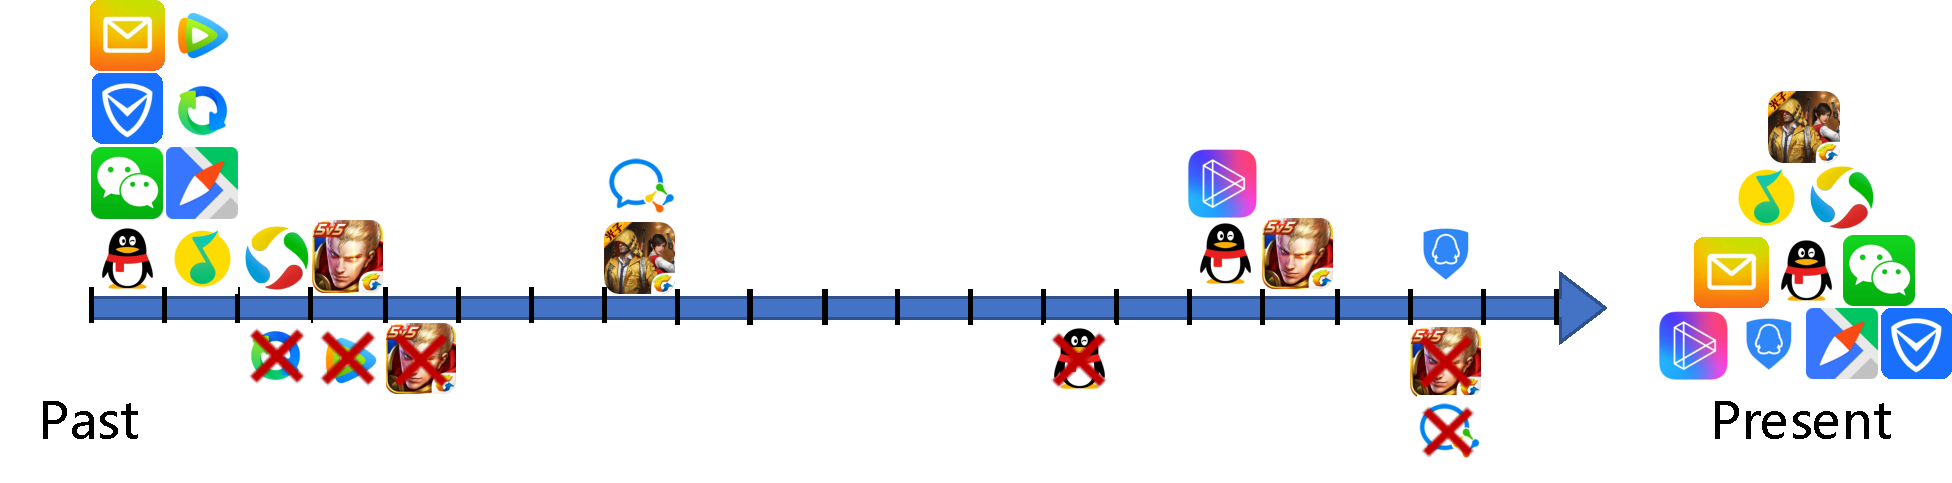
\includegraphics[width=0.8\linewidth]{figures/behaviors.pdf}
  \caption{\footnotesize{Illustration of retention, installation, and uninstallation. Operations of (un)installation are low-frequency and unevenly distributed over time.}}
  \label{fig:behaviors}
\end{figure}

При решении приктических задач, таких как рекомендации, предсказание вероятности клика (CTR prediction), поиск релевантной аудитории (lookalike), можно получить дополнительный прирост качества при использовании информации об использовании пользователем мобильных приложений.

Как правило, данную информацию добавляют в модели путем feature engineering'а, что может быть довольно сложно.  \\

В работе представлена модель, которая по данным об использовании приложений, позволяет построить General-Purpose эмбеддинг для пользователя.

Полученные эмбеддинги можно легко использовать для решения практических задача, избегая сложного feature engineering'а.

\section*{Как решают?}

Модель описанная в работе довольно сложная, поэтому мне бы хотелось рассмотреть один из бэйслайнов, приведенных в работе, который, не смотря на свою простоту, позволяет получать очень хорошие результаты.

\paragraph{Основная идея} Эмбеддинги для пользователя можно получить если скормить список установленных приложений в DAE (см. Рисунок~\ref{fig:dae}).

\begin{figure}[ht]
    \centering
    \begin{tikzpicture}

	\node (1) [draw, dashed, minimum height=15em, minimum width=15em, xshift=6.5em, fill=olivegreen, fill opacity=0.2, very thick, rectangle, rounded corners] {};
	\node (la1) [below=0em of 1] {\emph{encoder}};
	\node (2) [draw, dashed, minimum height=14em, fill = red, fill opacity=0.2,minimum width=14em, xshift=19em, very thick, rectangle, rounded corners] {};
	\node (la1) [below=0em of 2] {\emph{decoder}};
	\node (3) [draw, dashed, minimum height=16em, fill = blue, fill opacity=0.2,minimum width=5em, xshift=-1.5em, very thick, rectangle, rounded corners] {};
		\node (la3) [below=0em of 3] {\emph{corrupt}};
	
	\node[circle, thick, fill=red!50, draw] (x1) {};
	\node[circle, thick, draw, fill=red!50, below=1em of x1] (x2) {};
	\node[circle, thick, fill=red!50, draw, below=1em of x2] (x3) {};
	\node[circle, thick, fill=red!50, draw, below=1em of x3] (x4) {};
	\node[circle, thick, fill=red!50, draw, above=1em of x1] (x5) {};
	\node[circle, thick, fill=red!50, draw, above=1em of x5] (x6) {};
	\node[circle, thick, fill=red!50, draw, above=1em of x6] (x7) {};
	
	\foreach \x in {1,...,7}
		\node at (x\x) (lx\x) {$\sim$};
		
	\node[circle, thick, fill=white, left=2em of x1, draw] (i1) {};
	\node[circle, thick, draw, fill=white, below=1em of i1] (i2) {};
	\node[circle, thick, fill=white, draw, below=1em of i2] (i3) {};
	\node[circle, thick, fill=white, draw, below=1em of i3] (i4) {};
	\node[circle, thick, fill=white, draw, above=1em of i1] (i5) {};
	\node[circle, thick, fill=white, draw, above=1em of i5] (i6) {};
	\node[circle, thick, fill=white, draw, above=1em of i6] (i7) {};
	
	\foreach \x in {1,...,7}
		\draw[-stealth, decoration={snake, pre length=0.01mm, segment length=2mm, amplitude=0.3mm, post length=1.5mm}, decorate, thick] (i\x) -- (x\x);
	
	\node[circle, thick, right=4em of x1, fill=white, draw] (xh1) {};
	\node[circle, thick, draw, fill=white, below=1em of xh1] (xh2) {};
	\node[circle, thick, fill=white, draw, below=1em of xh2] (xh3) {};
	\node[circle, thick, fill=white, draw, above=1em of xh1] (xh4) {};
	\node[circle, thick, fill=white, draw, above=1em of xh4] (xh5) {};
	\node[circle, thick, fill=white, draw, right=8em of x1, yshift=5em] (hm1) {};
	\node[circle, thick, draw, fill=white, below=0.5em of hm1] (hm2) {};
	\node[circle, thick, draw, fill=white, below=0.5em of hm2] (hm3) {};
	\node[circle, thick, draw, fill=white, above=0.5em of hm1] (hm4) {};
	\node[circle, thick, fill=white, draw, right=8em of x1, yshift=-3em] (hs1) {};
	\node[circle, thick, draw, fill=white, below=0.5em of hs1] (hs2) {};
	\node[circle, thick, draw, fill=white, below=0.5em of hs2] (hs3) {};
	\node[circle, thick, draw, fill=white, above=0.5em of hs1] (hs4) {};
	\node[] at (hm1) (mu1) {$\mu$};
	\node[] at (hm2) (mu2) {$\mu$};
	\node[] at (hm3) (mu3) {$\mu$};
	\node[] at (hm4) (mu4) {$\mu$};
	\node[] at (hs1) (s1) {$\sigma$};
	\node[] at (hs2) (s2) {$\sigma$};
	\node[] at (hs3) (s3) {$\sigma$};
	\node[] at (hs4) (s4) {$\sigma$};
		
	\node[circle, thick, fill=lightgray, draw, right=12em of x1, yshift=1em] (h1) {};
	\node[circle, thick, draw, fill=lightgray, below=1em of h1] (h2) {};
	\node[circle, thick, draw, fill=lightgray, below=1em of h2] (h3) {};
	\node[circle, thick, draw, fill=lightgray, above=1em of h1] (h4) {};
	\node[circle, thick, right=16em of x1, fill=white, draw] (oh1) {};
	\node[circle, thick, draw, fill=white, below=1em of oh1] (oh2) {};
	\node[circle, thick, fill=white, draw, below=1em of oh2] (oh3) {};
	\node[circle, thick, fill=white, draw, above=1em of oh1] (oh4) {};
	\node[circle, thick, fill=white, draw, above=1em of oh4] (oh5) {};
	\node[circle, thick, draw, fill=white, right=20em of x1] (o1) {};
	\node[circle, thick, draw, fill=white, below=1em of o1] (o2) {};
	\node[circle, thick, draw, fill=white, below=1em of o2] (o3) {};
	\node[circle, thick, draw, fill=white, below=1em of o3] (o4) {};
	\node[circle, thick, draw, fill=white, above=1em of o1] (o5) {};
	\node[circle, thick, draw, fill=white, above=1em of o5] (o6) {};
	\node[circle, thick, draw, fill=white, above=1em of o6] (o7) {};
	\node[circle, thick, draw, fill=white, right=24em of x1] (oo1) {};
	\node[circle, thick, draw, fill=white, below=1em of oo1] (oo2) {};
	\node[circle, thick, draw, fill=white, below=1em of oo2] (oo3) {};
	\node[circle, thick, draw, fill=white, below=1em of oo3] (oo4) {};
	\node[circle, thick, draw, fill=white, above=1em of oo1] (oo5) {};
	\node[circle, thick, draw, fill=white, above=1em of oo5] (oo6) {};
	\node[circle, thick, draw, fill=white, above=1em of oo6] (oo7) {};
	\node[] at (o1) (muu1) {$\mu$};
	\node[] at (o2) (muu2) {$\mu$};
	\node[] at (o3) (muu3) {$\mu$};
	\node[] at (o4) (muu4) {$\mu$};
	\node[] at (o5) (muu5) {$\mu$};
	\node[] at (o6) (muu6) {$\mu$};
	\node[] at (o7) (muu7) {$\mu$};
	
	\foreach \x in {1,...,7}
		\foreach \y in {1,...,5}
			\draw[-stealth, thick] (x\x) -- (xh\y);
	
	\foreach \x in {1,...,5}
		\foreach \y in {1,...,4}
			\draw[-stealth, thick] (xh\x) -- (hm\y);
	
	\foreach \x in {1,...,5}
		\foreach \y in {1,...,4}
			\draw[-stealth, thick] (xh\x) -- (hs\y);
	
	\foreach \x in {1,...,4}
		\draw[-stealth, decoration={snake, pre length=0.01mm, segment length=2mm, amplitude=0.3mm, post length=1.5mm}, decorate, thick] (hs\x) -- (h\x);
	\foreach \x in {1,...,4}
		\draw[-stealth, decoration={snake, pre length=0.01mm, segment length=2mm, amplitude=0.3mm, post length=1.5mm}, decorate, thick] (hm\x) -- (h\x);
	
	\foreach \x in {1,...,5}
		\foreach \y in {1,...,4}
			\draw[-stealth, thick] (h\y) -- (oh\x);
	
	\foreach \x in {1,...,5}
		\foreach \y in {1,...,7}
			\draw[-stealth, thick] (oh\x) -- (o\y);
				
	\foreach \x in {1,...,7}
		\draw[-stealth, decoration={snake, pre length=0.01mm, segment length=2mm, amplitude=0.3mm, post length=1.5mm}, decorate, thick] (o\x) -- (oo\x);
				
	\node[left=0.5em of i1] (l1) {$\vec{x}$};
	\node[above=0em of h4] (l2) {$\vec{z}$};
	\node[right=0.5em of oo1] (l3) {$\vec{x}'$};

\end{tikzpicture}
    \caption{\footnotesize{Denoising Autoencoder (DAE)}}
    \label{fig:dae}
\end{figure}

\paragraph{Data Preprocessing} Прежде обучать модель, нужно выполнить предварительную чистку данных, чтобы эмбеддинги пользователей лучше отражали их интересы:
\begin{itemize}
    \item Игнорируются наиболее популярные приложения, которые есть практически на всех смартфонах, так как факт их наличия на телефоне мало что говорит об интересах пользователя
    \item Игнорируются предустановленные на телефон приложения
    \item Также исключаются совсем редкие приложения, которые установлены у маленького числа пользователей
\end{itemize}

\subsection*{Experiments}

В статье представлен ряд экспериментов, подтверждающих полезность полученных эмбеддингов пользователей.

Рассмотрим два эксперимента

\paragraph{Test \#1: Next Week’s Installation Prediction} В рамках первого теста, эмбеддинги пользователя используют для предсказания того какие приложения пользователь установит в течении следующей недели.

Для решения задачи обучают нейросеть, состоящую из нескольких полносвязных слоев, на эмбеддингах пользователей.

\paragraph{Test \#2: Look-alike Audience Extension} В рамках второго теста, эмбеддинги используются для расширения аудитории.

Данные для обучения --- аудитория из миллиона пользователей, примерно 10\% из которых - seed (пользователи, которые используют некоторое нишевое приложение). 

Задача состоит в том, чтобы научиться искать пользователей, похожих на seed. 

Для этого на эмбеддингах пользователей обучается классификатор (XGBoost), который предсказывает вероятность того, что пользователь относится к seed пользователям. \\

В качестве метрики для оценки качества использовали ROC AUC. \\

Не смотря на простоту подхода, использование DAE показывает результаты, которые не намного хуже в сравнении с моделью описанной в статье.

\section*{Преимущества подхода}

\begin{itemize}
    \item Простой в реализации подход
    \item Не требует частого переобучения модели целиком, так как новые приложения появляются не так часто
    \item Позволяет практически в онлайне обновлять эмбеддинги для пользователей при установке/удаление приложений, что позволяет лучше реагировать на изменение интересов пользователя
\end{itemize}